
\newcommand{\FigOverview}{
\begin{figure}[t]
    \centering
    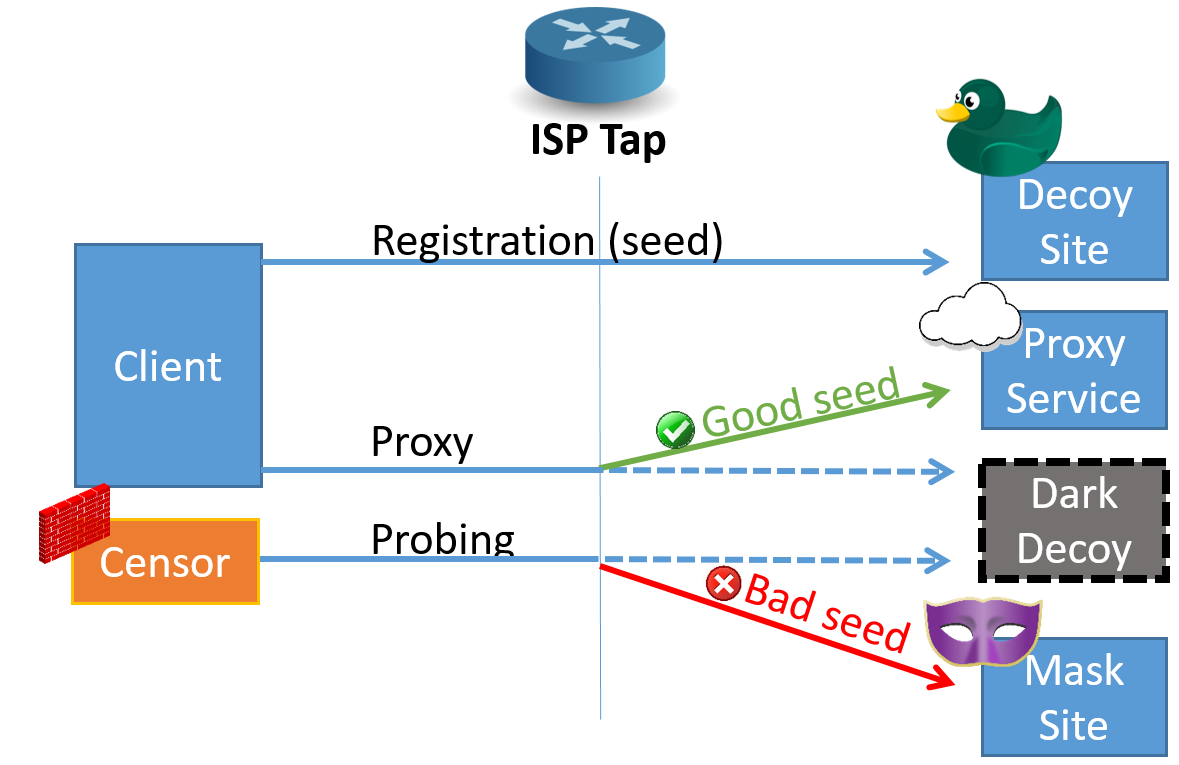
\includegraphics[width=\linewidth,clip]{figures/dark-decoy-overview.png}
    \caption{\textbf{\scheme Operations}\,---\,%
        Clients first register by sending a secret seed in a steganographic tag past the station in a
        normal TLS connection to a Decoy site. Clients then connect to an address derived from the seed,
        which the station responds as a phantom host. If the client can prove knowledge of the
        seed used during registration, they are allowed access to the proxy. Otherwise,
        their traffic is forwarded to a Mask Site to make it difficult for censors to distinguish
        phantom hosts from legitimate ones.
    }
    \label{fig:overview}
\end{figure}
}

\newcommand{\FigHighLevel}{
\begin{figure}[t]
    \centering
    \vspace{-0.54in}
    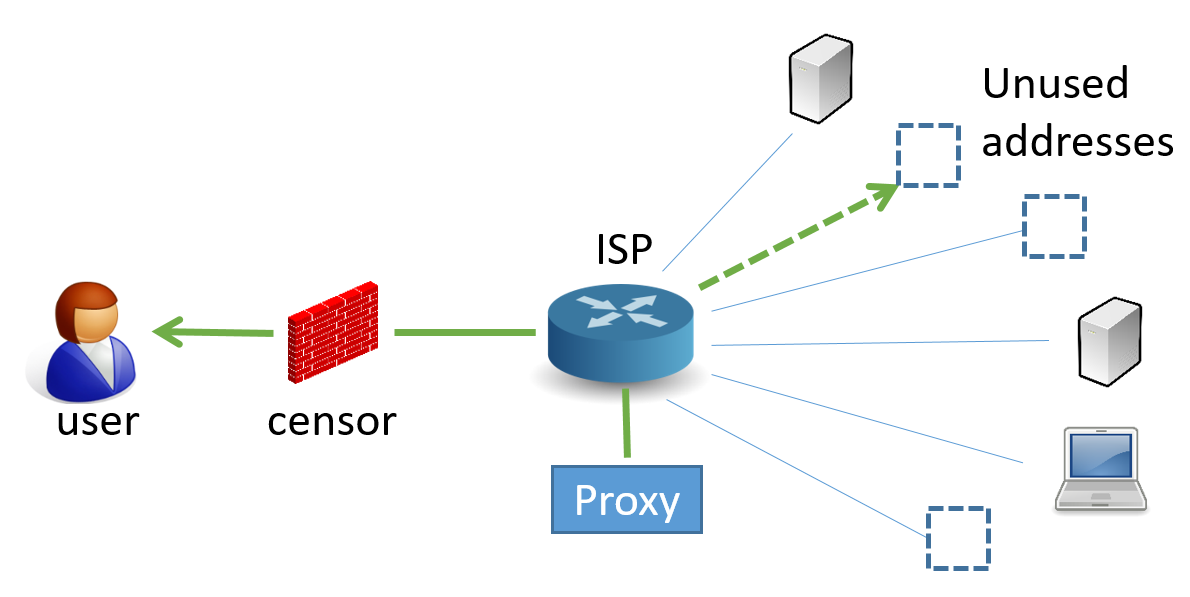
\includegraphics[width=\linewidth,clip]{figures/high-level.png}
    \caption{\textbf{\scheme Overview}---%
      An ISP deploys a \scheme station, which sees a passive tap of passing traffic.
      Following a steganographic registration process, a client can connect
      to an unused IP address in the ISP's AS, and the station will
      inject packets to communicate with the client as if there were a proxy server at that address.
    }
    \label{fig:highlevel}
\end{figure}
}

\newcommand{\FigUpload}{
\begin{figure}[t]
    \centering
    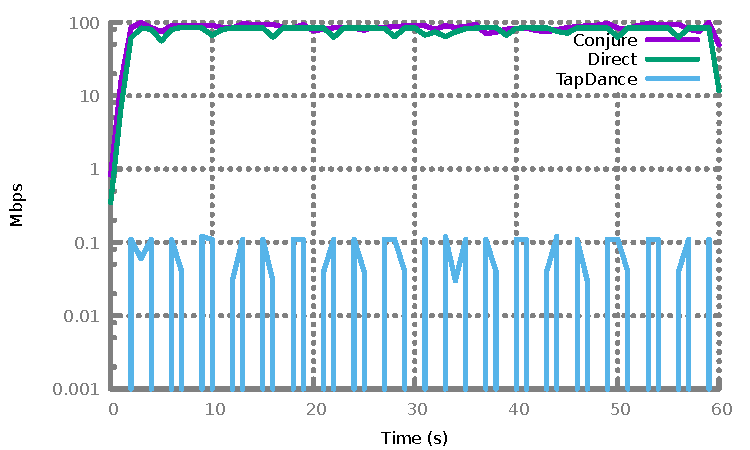
\includegraphics[width=0.95\linewidth,clip]{figures/bandwidth-up.pdf}
    \caption{\textbf{Upload Performance}\,---\, %
        We used iperf to measure the upload bandwidth for a direct connection, TapDance, and \scheme.
        As expected, TapDance's upload performance is several orders of magnitude lower than
        the link capacity, due to the overhead of frequent reconnects to the decoy.
    }
    \label{fig:upload}
\end{figure}
}

\newcommand{\FigDownload}{
\begin{figure}[t]
    \centering
    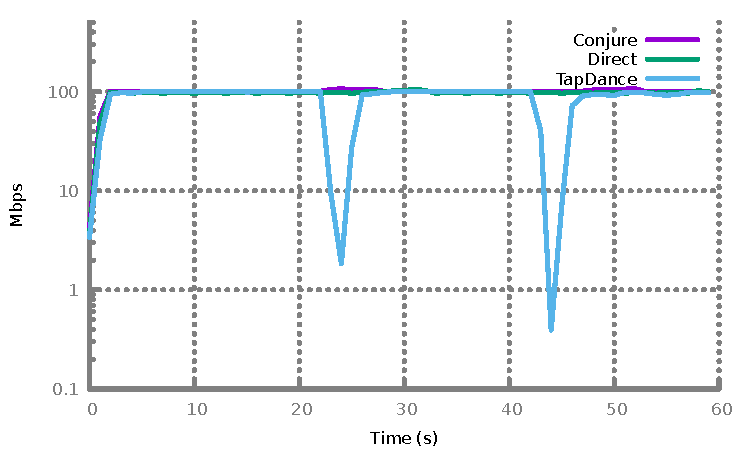
\includegraphics[width=0.95\linewidth,clip]{figures/bandwidth-down.pdf}
    \caption{\textbf{Download Performance}\,---\, %
        Using iperf, we compare the download performance of a direct connection, TapDance, and \scheme.
        While TapDance can achieve link capacity download, it still has to occasionally reconnect
        to the decoy, as seen by the periodic dips. These reconnects are more common the more data
        the client sends (e.g. requests or any upload data).
    }
    \label{fig:download}
\end{figure}
}


\newcommand{\FigTapBandwidth}{
\begin{figure*}[ht]
    \centering
    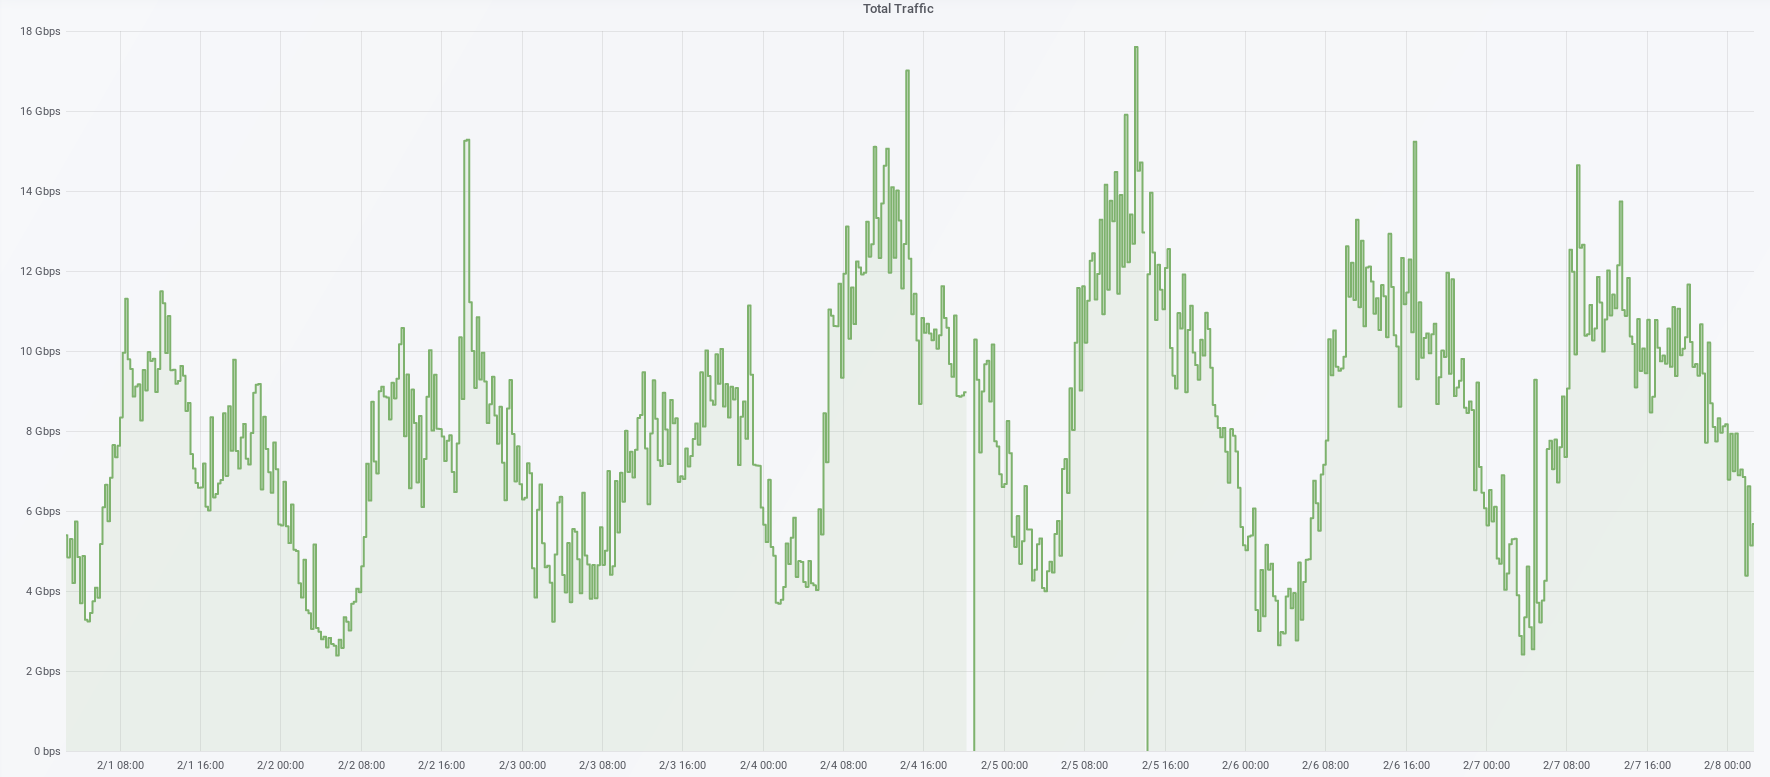
\includegraphics[width=0.75\linewidth,clip]{figures/decoy-tap-bandwidth.png}
    \caption{\textbf{Tap Bandwidth}\,---\, %
        We deployed our \scheme implementation in a realistic ISP testbed on a
        (full duplex) tap of a 10~Gbps router. As shown in a typical week, traffic
        ranges from 2-17~Gbps.
    }
    \label{fig:tap-bandwidth}
\end{figure*}
}




\newcommand{\FigIpBits}{
\begin{figure}[t]
    \centering
    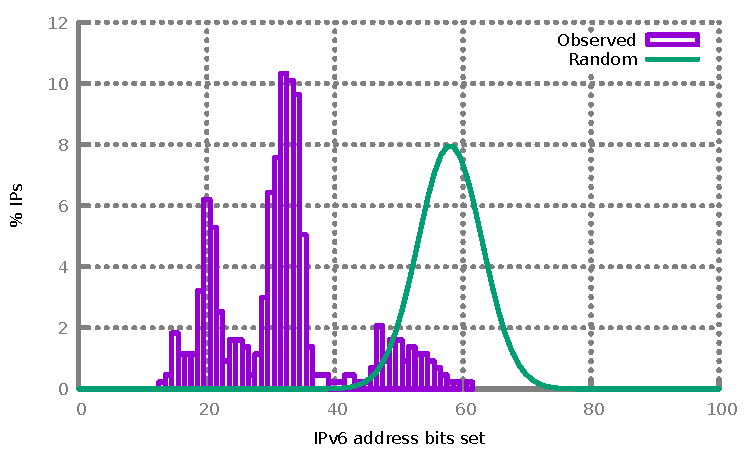
\includegraphics[width=\linewidth,clip]{figures/ip-bits-set-pdf.pdf}
    \caption{\textbf{IPv6 Entropy}---%
        We observed 30 minutes of IPv6 traffic on our tap to the /32 of the ISP's network.
        In each address observed, we counted the number of bits set, and compared this to
        randomly generated addresses. If the 96 non-network bits
        of each address were chosen randomly, we would expect to see a Binomial distribution
        (shown as Random). In practice, the distribution of observed IP addresses has much fewer
        bits set, suggesting that censors might be able to distinguish between phantom host addresses
        and legitimate ones.\looseness=-1
        %We note there are several /64 subnets that had many
        %addresses that appeared random (visibly overlapping the random distribution).
    }
    \label{fig:ipbits}
\end{figure}
}





\newcommand{\yes}{\CIRCLE}
\newcommand{\no}{\Circle}
\newcommand{\maybe}{\LEFTcircle}

\newcommand{\TabCompare}{
\begin{table*}[t]
    \centering
    \begin{tabular}{l|cccccccc}
            % Multiflow? Waterfall?
            & \rot{Telex~\cite{telex11}} &
            \rot{Cirripede~\cite{cirripede11}} &
            \rot{Decoy Routing~\cite{curveball11}} &
            \rot{TapDance~\cite{tapdance14}} & \rot{Rebound~\cite{rebound15}} & \rot{Slitheen~\cite{slitheen16}} & \rot{Waterfall~\cite{waterfall17}} & \rot{\textbf{\scheme}} \\
            \hline
                                      %Telex Cirr  DR     TD      RB    Slth   Water  DD
            No inline blocking        & \no & \no  & \no & \yes  & \no  & \no  & \no  & \yes \\
            Handles asym.\ routing     & \no & \yes & \no  & \yes & \yes & \no  & \yes & \yes \\
            %Currently deployed        & \no & \no  & \no  & \yes & \no  & \no  & \no  & \no \\
            Replay attack resistant   &\yes & \yes & \yes & \no  & \yes & \yes & \yes & \yes \\
            Traffic analysis resistant &\no  & \no  & \no  & \no  &\maybe& \yes &\maybe& \no \\
            %Uses unused addresses     & \no & \no  & \no  & \no  & \no  & \no  & \no  & \yes \\
            Unlimited Session Length  &\yes & \yes & \yes & \no  & \no  & \no  & \no  & \yes \\
            %Multicore Implementation  &\no  & \no  & \no  & \yes & \no  & \no  & \no  & \yes \\
    \end{tabular}
    \caption{\textbf{Comparing Refraction Networking schemes}\,---\,
        ``No inline blocking'' corresponds to schemes that can operate as a passive tap on the side
        without needing an inline element in the ISP network.
        ``Handles asymmetric routes'' refers to schemes that work when only one direction (either client to decoy or decoy to server) is seen by the station.
        ``Replay attacks'' refers to censors who may replay/preplay previous messages or actively probe
        the protocol.
        ``Traffic analysis'' includes latency, inter-packet timing, and website fingerprinting.
        ``Unlimited Sessions'' shows schemes that do not need to repeatedly reconnect to download
        or upload arbitrarily large content.}
    \label{tab:compare}
\end{table*}
}



\newcommand{\FigImplementation}{
\begin{figure}[t]
    \centering
    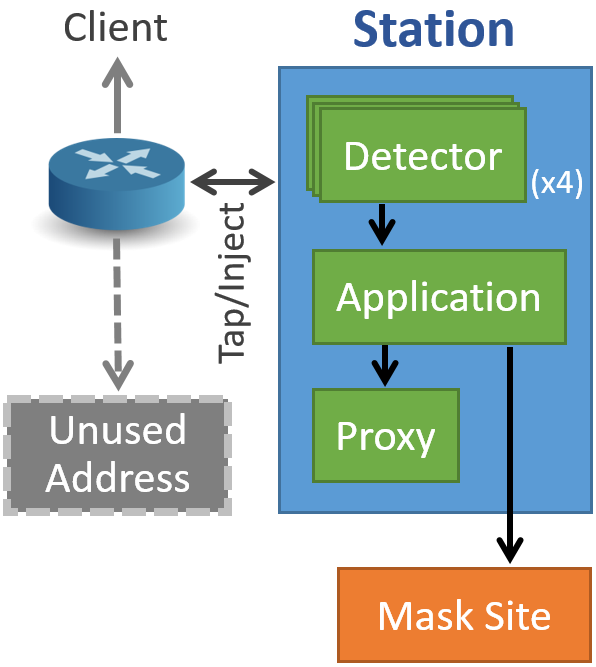
\includegraphics[width=0.7\linewidth,clip]{figures/implementation.png}
    \caption{\textbf{Station Architecture}\,---\,%
        We used PF\_RING to receive packets from a 10~Gbps packet tap, which we load balance
        across 4~CPU cores. The detector process identifies and processes registrations, and forwards
        packets destined to registered dark decoy addresses to a local application. The application
        determines if the client is legitimate (using a seed shared during registration) and forwards
        their traffic to a proxy. Otherwise, the application responds as if it were the mask site.
    }
    \label{fig:implementation}
\end{figure}
}

\newcommand{\FigEvolution}{
\begin{figure}
  \centering
  \begin{subfigure}{\columnwidth}
    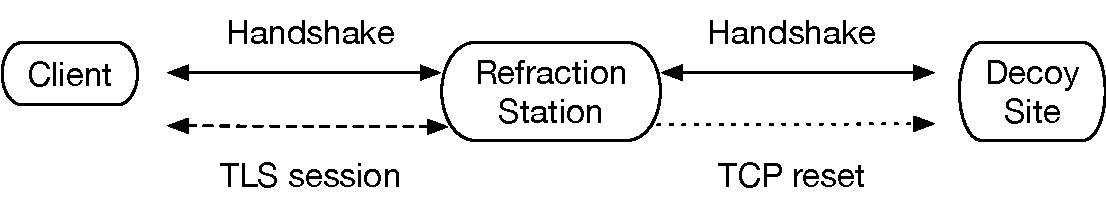
\includegraphics[width=\columnwidth]{figures/refraction-v1}
    \vspace{-3pt}

    \caption{\textbf{First generation systems} for Refraction Networking, such as Telex and Cirripede, operated as inline network elements, with the ability to observe traffic and block specific flows. ISPs worried that if the inline element failed, it could bring down the network.\looseness=-1}
    \label{fig:refraction-v1}
  \end{subfigure}
  \vspace{16pt}

  \begin{subfigure}{\columnwidth}
    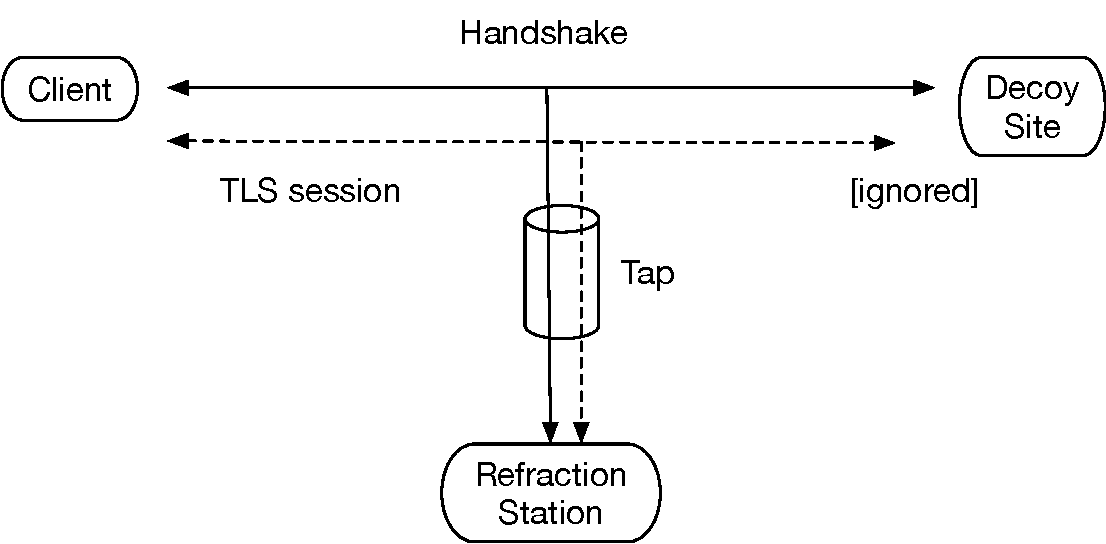
\includegraphics[width=\columnwidth]{figures/tapdance}
    \vspace{-3pt}

    \caption{\textbf{TapDance} is a second-generation Refraction Network scheme that operates without flow blocking, needing only to passively observe traffic and inject packets. TapDance has recently been deployed at a mid-size ISP, but the techniques used to silence the decoy site and participate in the client--decoy TCP connection mid-stream add significant complexity, performance bottlenecks, and detection risk.}
    \label{fig:tapdance}
  \end{subfigure}
  \vspace{16pt}

  \begin{subfigure}{\columnwidth}
    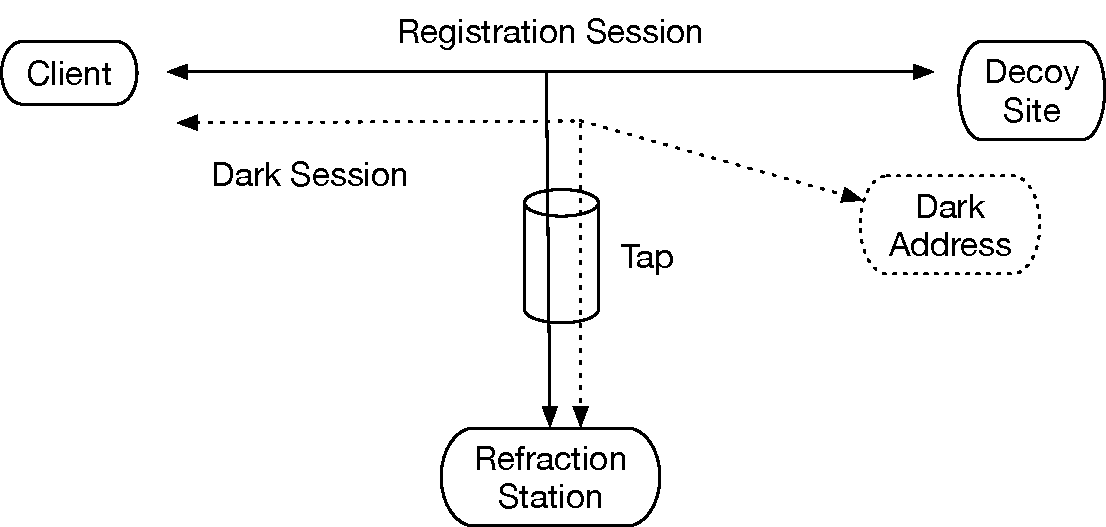
\includegraphics[width=\columnwidth]{figures/dark-decoys}
    \vspace{-3pt}

    \caption{\textbf{\scheme}, our third-generation Refraction Networking design, overcomes these limitations.  It uses two sessions. First, the client connects to a decoy site and embeds a steganographic registration message, which the station receives using only a passive tap.  Second, the client connects to a ``phantom host'' where there is no running server, and the station proxies the connection in its entirety.}
    \label{fig:dark-decoys}
  \end{subfigure}

  \vspace{12pt}
  \caption{\textbf{Evolution of Refraction Networking}}
\end{figure}
}
